\def\x{x}
\def\Q{Q}
\def\bds#1{#1}
\def\tts#1{\texttt{\small #1}}

\section{Experiments}
\label{sec:thesims}

We perform both synthetic and real data experiments.

\subsection{Simulations}
We first illustrate our methods using a simulation of the model
\begin{equation}\nonumber
         Y_i = f_o(\x_{iS}) + \epsilon_i \quad (i=1,2,\ldots,n).
\end{equation}
Here $\x_{i}$ denotes data sample $i$ drawn from some distribution $P$. 
$\x_{iS}$ is a subset of $\x_i$ with dimension $|S|=s$, where $S$
represents the set of relevant variables, and 
$\epsilon_i$ is additive noise drawn from $\mathcal{N}(0,\sigma)$. For 
all simulations, we set $\sigma$ such that the signal-to-noise ratio(SNR, $\frac{\trm{std}(Y)}{\sigma}$) is 5; we
set $\lambda = \frac{1}{2} \sqrt{ \frac{\log^2(np)}{n} }$.

For the first three simulations, we will use the quadratic form as our true regression function.
\[
f_0(x_{iS}) = x_{iS}^\tran \Q x_{iS}
\]

The matrix $\Q$ is a symmetric positive definite matrix of dimension $|S|\times{}|S|$. 
Note that if $\Q$ is diagonal, then the true function is convex
additive; 
otherwise the true function is convex but not additive.

In the \textbf{first simulation}, we vary the ambient dimension $p$. We set $Q$ as one on the diagonal and $1/2$ on the off-diagonal with $0.5$ probability, and choose $n=100, 200,\ldots,1000$ and $p=64,128,256$ and $512$. We use independent $X$ and draw $X \sim N(0, I_p)$.
For each $(n,p)$ combination, we generate $100$ independent data
sets. For each data set we use the AC/DC algorithm and mark feature $j$ as irrelevant if both the AC estimate $\| \hat{f}_j \|_\infty$ and the DC estimate $\| \hat{g}_k \|_\infty$ are smaller than $10^{-6}$.
We plot the probability of exact
support recovery over the $100$ independent trials in Figure \ref{Support}(a).  We
observe that the algorithm performs consistent variable selection even if the dimensionality is large. To give the reader a
sense of the running speed, for a 
data set with $n=1000$ and $p=512$, the code runs in roughly two 
minutes on a machine with 2.3 GHz Intel Core i5 CPU and 4 GB memory.

In the \textbf{second simulation}, we vary the sparsity of the $Q$ matrix, that is, we vary the extent to which the true function is non-additive. We generate four $\Q$ matrices
plotted in Figure \ref{Support}(c), where the diagonal elements are all one and
the off-diagonal elements are $\frac{1}{2}$ with probability $\alpha$
($\alpha=0,0.2,0.5,1$ for the four cases). We show the 4 $\Q$ matrices we used in Figure~\ref{Support}(c).
We fix $p=128$ and choose
$n=100,200,\ldots,1000$. We use $X \sim N(0,I_p)$. We again run the AC/DC optimization on $100$
independent trials and plot the probability of recovery
in Figure \ref{Support}(b). The results demonstrate that AC/DC performs
consistent variable selection even if the true function is not additive (but
still convex).

In the third, fourth, and fifth simulations, we use correlated design and vary the correlation. We generate $X$ from a non-Gaussian correlated boundary flat distribution. The distribution we used is a mixture of a uniform distribution and a Gaussian Copula.
\[
X \sim \gamma U([-2, 2]^p) + (1-\gamma) \trm{Copula}(0, \Sigma, F)
\]
Gaussian Copula is a way to customize the marginal distributions of a Gaussian random variable while maintaining the covariance structure. Gaussian Copula results when one applies a monotone transformation $F^{-1} \Phi$ onto each variable of Gaussian random vector where $\Phi$ is the normal CDF and $F$ is the CDF of the new desired marginal distribution. In all our experiments, we set $\gamma = 0.05$ and set the marginal CDF $F$ so that marginal density of the Copula is bimodal and supported on $[-1.8, 1.8]$. The marginal density of the mixture is shown in Figure~\ref{fig:copula_marginal}. Notice that boundary flatness holds because the distribution is uniform in the boundary area $[-2,2]^p \backslash [-1.8, 1.8]^p$.

\begin{figure*}
\includegraphics[width=.4\textwidth]{figs/copula_marginal}
\caption{Marginal density of the Gaussian Copula and Uniform Mixture}
\label{fig:copula_marginal}
\end{figure*}

In the \textbf{third experiment}, we set $\Sigma_{ij}=\nu^{|i-j|}$ for $\nu = 0, 0.2, 0.5, 0.9$. We use the non-additive $\Q$, same as in the first experiment, with $\alpha=0.5$ and fix $p=128$. We measure success not through exact recovery but through approximate recovery. We say that a trial is a successful if (1) all relevant variables were recovered and (2) fewer than $20$ variables were marked as relevant overall. The probabilities of success are computed from 40 independent trials and plotted against various values of $\nu$ in Figure~\ref{Support}(d). Additionally, for $\nu = 0.5$, we show the number of selected variables versus the sample size as a Box-and-Whisker plot in Figure~\ref{Support}(e). As can be seen, AC/DC can successfully recover the relevant variables with only a small number of false positives. 

In the fourth, fifth, and sixth simulation, we use a softmax regression function
\[
f_0(x_{iS}) = \log \left( \sum_{k=1}^K \exp( \beta_k^\tran x_{iS} ) \right) - \mu
\]
where $\{\beta_k \in \R^s\}_{k=1,...,K}$ are random unit vectors. $\mu$ is chosen so that $f_0$ has mean-zero. We set $K = 7$ for all the experiments. 

For the \textbf{fourth experiment}, we use the softmax regression function and $X$ drawn from the boundary flat mixture distribution described earlier with correlation level $\nu = 0.5$. We use the same approximate recovery success criteria as the third experiment and plot probability of approximate recovery against the number of samples for $p=128, 256, 512$. The probabilities are computed over 30 independent trials. 

For the \textbf{fifth experiment}, we use the softmax regression function and $X$ drawn from the boundary flat mixture distribution with correlation level $\nu = 0.2$. 

For the \textbf{sixth experiment}, we compare the variables selected via the AC stage and the variables selected via the DC stage. We use the softmax regression function and $X$ drawn from the boundary flat mixture distribution with correlation level $\nu = -0.7$. We set $n=500, p=128$. We perform 30 independent trials and plot the frequency of variable selection in Figure~\ref{fig:ac_v_dc}. The true variables are $X_j$ for $j=5,6,7,8,9,10$. We plot the frequency of selection among only the first 20 variables, that is, $X_j$ for $j=1,...,20$. We do not plot selection frequencies for variables 21 to 128 because they are almost never selected by either AC or DC. As can be seen, the DC stage is slightly helpful in recovering the true variables but its effect is not significant. We thus believe that the DC stage, though important in theory, is not as important in practice; it may be omitted without significant detriment to the overall result. 

\begin{figure*}[!t]
\begin{center}
\begin{tabular}{cc}
%\hskip-10pt
\includegraphics[width=.42\textwidth]{figs/CurveT} &
%\hskip-10pt
\includegraphics[width=.42\textwidth]{figs/CurveR} \\
(a) quadratic $f_0$, independent $X$, varying $p$  & (b) quadratic $f_0$, independent $X$, varying $\Q$ \\
%\hskip-10pt
\includegraphics[width=.42\textwidth]{figs/Q} &
%\hskip-10pt
\includegraphics[width=.42\textwidth]{figs/CurveC}  \\
(c) four $\Q$ matrices used in (b) & (d) quadratic $f_0$, correlated $X$, varying correlation $\nu$ \\
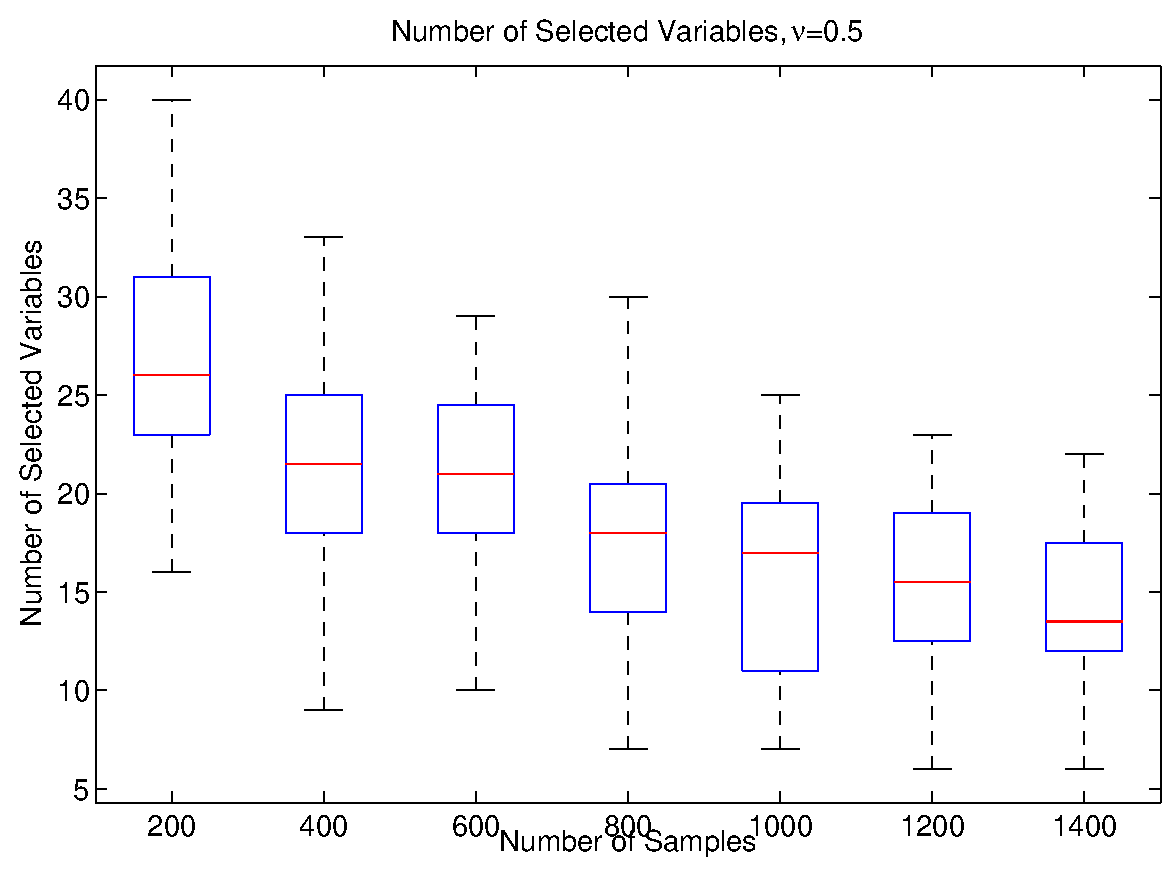
\includegraphics[width=.42\textwidth]{figs/C_support_box} & 
\includegraphics[width=.42\textwidth]{figs/CurveS}\\
(e) recovered support size for $\nu=0.5$ in (d) & (f) softmax $f_0$, correlated $X$, varying $p$ \\
\includegraphics[width=0.42\textwidth]{figs/S_support_box} & \\
(g) recovered support size for $p=256$ in (f) & (h) softmax $f_0$, correlated $X$, varying $s$ 
\end{tabular}
\end{center}
\caption{Support recovery results where the additive assumption is
  correct (a), incorrect (b), (c), and with correlated design (d).}\label{Support}
\vskip10pt
\end{figure*}

\begin{figure*}
\includegraphics[width=0.5\textwidth]{figs/ACvDC}
\caption{Frequency of variable selection among the first 20 variables ($X_j$ for $j=1,...,20$) in the AC stage vs. in the DC stage. The true variables are [5,6,7,8,9,10].}
\label{fig:ac_v_dc}
\end{figure*}


\subsection{Boston housing data}

We next use the Boston housing data rather than simulated data. This data set
contains 13 covariates, 506 samples and one response variable
indicating housing values in suburbs of Boston. The data and detailed description
can be found on the UCI Machine Learning Repository website\footnote{\url{http://archive.ics.uci.edu/ml/datasets/Housing}}. 

We first use all $n=506$ samples (with standardization) in the AC/DC algorithm,
using a set of candidate regularization parameters $\{\lambda^{(t)}\}$
ranging from $\lambda^{(1)} = 0$ (no regularization) to $2$. For each $\lambda^{(t)}$
we obtain a function value matrix $\bds{f}^{(t)}$ with $p=13$
columns and $n=506$ rows. The non-zero columns in this matrix indicate the variables selected using $\lambda^{(t)}$.  

In Figure~\ref{Boston}(a), we plot on the y-axis the norm $\|\bds{f}^{(t)}_j\|_{\infty}$ of every column $j$ against the regularization strength $\lambda^{(t)}$. Instead of plotting the value of $\lambda^{(t)}$ on the x-axis however, we plot the total norm at $\lambda^{(t)}$ normalized against the total norm at $\lambda^{(1)}$: $\frac{\sum_j \|\bds{f}^{(t)}_j\|_{\infty}}{\sum_j \|\bds{f}^{(1)}\|_{\infty}}$. Thus, as x-axis moves from 0 to 1, the regularization goes from strong to weak. For comparison, we
plot the LASSO/LARS result in a similar way in Figure \ref{Boston}(b).
From the figures we observe that the first three variables selected by
AC/DC and LASSO are the same: \tts{LSTAT}, \tts{RM} and \tts{PTRATIO},
consistent with previous findings~\citep{SpAM:07}.  The fourth
variable selected by AC/DC is \tts{INDUS} (with $\lambda^{(t)}=0.7$).
We then refit AC/DC with only these four variables without
regularization, and plot the estimated additive functions in Figure
\ref{Boston}(d). When refitting, we constrain a component to be convex if it is non-zero in the AC stage and concave if it is non-zero in the DC stage. As can be seen, these functions contain clear
nonlinear effects which cannot be captured by LASSO. The shapes of
these functions, including the concave shape of the \tts{PTRATIO} function, are in agreement with those obtained by
SpAM~\citep{SpAM:07}. 

Next, in order to quantitatively study the predictive performance, we
run 3 times 5-fold cross validation, following the same procedure
described above---training, variable selection and refitting.  A plot
of the mean and standard deviation of the predictive mean squared
error (MSE) is shown in Figure \ref{Boston}(c). Since for AC/DC the same
regularization level $\lambda^{(t)}$ may lead to a slightly different number of selected
variables in different folds and runs, the values on the $x$-axis
for AC/DC are not necessarily integers. The figure clearly shows that AC/DC has a 
lower predictive MSE than LASSO.  We also compared the performance of
AC/DC with that of Additive Forward Regression (AFR) presented
in~\cite{Xi:09}, and found that they are similar.  The main advantages
of AC/DC compared with AFR and SpAM are that there are no smoothing
parameters required, and the optimization is formulated
as a convex program, guaranteeing a global optimum.

%\begin{figure}[!htpb]
%        \centering
%        \begin{subfigure}[b]{0.45\textwidth}
%                \centering
%                \includegraphics[width=\textwidth]{figs/Additive}
%                 \caption{Variable selection result using AC/DC.}
%                \label{AC/DC}
%        \end{subfigure}
%        \begin{subfigure}[b]{0.45\textwidth}
%                \centering
%                \includegraphics[width=\textwidth]{figs/Additive1}
%                 \caption{Variable selection result using AC/DC.}
%                \label{AC/DC1}
%        \end{subfigure}\\
%        \begin{subfigure}[b]{0.45\textwidth}
%                \centering
%                \includegraphics[width=\textwidth]{figs/LASSO}
%                \caption{Variable selection result using LASSO.}
%                \label{LASSO}
%        \end{subfigure}
%        \begin{subfigure}[b]{0.45\textwidth}
%                \centering
%                \includegraphics[width=\textwidth]{figs/MSE}
%                 \caption{Predictive MSE of AC/DC and LASSO.}
%                 \label{MSE}
%        \end{subfigure}\\
%        \begin{subfigure}[b]{0.45\textwidth}
%                \centering
%                \includegraphics[width=\textwidth]{figs/Convex}
%                \caption{Inferred additive convex functions by AC/DC.}
%                \label{Convex}
%        \end{subfigure}
%        \caption{Results on Boston housing data.}\label{Boston}
%\end{figure}



\begin{figure*}
\begin{center}
\begin{tabular}{cc}
%\hskip-10pt
  \includegraphics[width=.38\textwidth]{figs/acdc_path}  &
%\hskip-25pt
  \includegraphics[width=.38\textwidth]{figs/lasso_path} 
\\
%\hskip-10pt 
(a) AC/DC $\|f_k\|_\infty$ paths & 
%\hskip-25pt
(b) LASSO $|\beta_k|$ paths \\
%\end{tabular}
%\begin{tabular}{cc}
  \includegraphics[width=.38\textwidth]{figs/MSEacdc} &
%\hskip 5pt
  \includegraphics[width=.45\textwidth]{figs/acdc_functs}
\\
(c) predictive MSE & (d) estimated functions from AC/DC
\end{tabular}
\end{center}
\caption{Results on Boston housing data, showing regularization paths,
 MSE and fitted functions.} \label{Boston}
\end{figure*}


% DO NOT CHANGE; RefTex variables -minx
 
%%% Local Variables: ***
%%% mode:latex ***
%%% TeX-master: "paper.tex" ***
%%% End: ***

